% Options for packages loaded elsewhere
\PassOptionsToPackage{unicode}{hyperref}
\PassOptionsToPackage{hyphens}{url}
%
\documentclass[
  man, donotrepeattitle,floatsintext]{apa6}
\usepackage{amsmath,amssymb}
\usepackage{lmodern}
\usepackage{iftex}
\ifPDFTeX
  \usepackage[T1]{fontenc}
  \usepackage[utf8]{inputenc}
  \usepackage{textcomp} % provide euro and other symbols
\else % if luatex or xetex
  \usepackage{unicode-math}
  \defaultfontfeatures{Scale=MatchLowercase}
  \defaultfontfeatures[\rmfamily]{Ligatures=TeX,Scale=1}
\fi
% Use upquote if available, for straight quotes in verbatim environments
\IfFileExists{upquote.sty}{\usepackage{upquote}}{}
\IfFileExists{microtype.sty}{% use microtype if available
  \usepackage[]{microtype}
  \UseMicrotypeSet[protrusion]{basicmath} % disable protrusion for tt fonts
}{}
\makeatletter
\@ifundefined{KOMAClassName}{% if non-KOMA class
  \IfFileExists{parskip.sty}{%
    \usepackage{parskip}
  }{% else
    \setlength{\parindent}{0pt}
    \setlength{\parskip}{6pt plus 2pt minus 1pt}}
}{% if KOMA class
  \KOMAoptions{parskip=half}}
\makeatother
\usepackage{xcolor}
\usepackage{graphicx}
\makeatletter
\def\maxwidth{\ifdim\Gin@nat@width>\linewidth\linewidth\else\Gin@nat@width\fi}
\def\maxheight{\ifdim\Gin@nat@height>\textheight\textheight\else\Gin@nat@height\fi}
\makeatother
% Scale images if necessary, so that they will not overflow the page
% margins by default, and it is still possible to overwrite the defaults
% using explicit options in \includegraphics[width, height, ...]{}
\setkeys{Gin}{width=\maxwidth,height=\maxheight,keepaspectratio}
% Set default figure placement to htbp
\makeatletter
\def\fps@figure{htbp}
\makeatother
\setlength{\emergencystretch}{3em} % prevent overfull lines
\providecommand{\tightlist}{%
  \setlength{\itemsep}{0pt}\setlength{\parskip}{0pt}}
\setcounter{secnumdepth}{-\maxdimen} % remove section numbering
% Make \paragraph and \subparagraph free-standing
\ifx\paragraph\undefined\else
  \let\oldparagraph\paragraph
  \renewcommand{\paragraph}[1]{\oldparagraph{#1}\mbox{}}
\fi
\ifx\subparagraph\undefined\else
  \let\oldsubparagraph\subparagraph
  \renewcommand{\subparagraph}[1]{\oldsubparagraph{#1}\mbox{}}
\fi
\newlength{\cslhangindent}
\setlength{\cslhangindent}{1.5em}
\newlength{\csllabelwidth}
\setlength{\csllabelwidth}{3em}
\newlength{\cslentryspacingunit} % times entry-spacing
\setlength{\cslentryspacingunit}{\parskip}
\newenvironment{CSLReferences}[2] % #1 hanging-ident, #2 entry spacing
 {% don't indent paragraphs
  \setlength{\parindent}{0pt}
  % turn on hanging indent if param 1 is 1
  \ifodd #1
  \let\oldpar\par
  \def\par{\hangindent=\cslhangindent\oldpar}
  \fi
  % set entry spacing
  \setlength{\parskip}{#2\cslentryspacingunit}
 }%
 {}
\usepackage{calc}
\newcommand{\CSLBlock}[1]{#1\hfill\break}
\newcommand{\CSLLeftMargin}[1]{\parbox[t]{\csllabelwidth}{#1}}
\newcommand{\CSLRightInline}[1]{\parbox[t]{\linewidth - \csllabelwidth}{#1}\break}
\newcommand{\CSLIndent}[1]{\hspace{\cslhangindent}#1}
\ifLuaTeX
\usepackage[bidi=basic]{babel}
\else
\usepackage[bidi=default]{babel}
\fi
\babelprovide[main,import]{english}
% get rid of language-specific shorthands (see #6817):
\let\LanguageShortHands\languageshorthands
\def\languageshorthands#1{}
% Manuscript styling
\usepackage{upgreek}
\captionsetup{font=singlespacing,justification=justified}

% Table formatting
\usepackage{longtable}
\usepackage{lscape}
% \usepackage[counterclockwise]{rotating}   % Landscape page setup for large tables
\usepackage{multirow}		% Table styling
\usepackage{tabularx}		% Control Column width
\usepackage[flushleft]{threeparttable}	% Allows for three part tables with a specified notes section
\usepackage{threeparttablex}            % Lets threeparttable work with longtable

% Create new environments so endfloat can handle them
% \newenvironment{ltable}
%   {\begin{landscape}\centering\begin{threeparttable}}
%   {\end{threeparttable}\end{landscape}}
\newenvironment{lltable}{\begin{landscape}\centering\begin{ThreePartTable}}{\end{ThreePartTable}\end{landscape}}

% Enables adjusting longtable caption width to table width
% Solution found at http://golatex.de/longtable-mit-caption-so-breit-wie-die-tabelle-t15767.html
\makeatletter
\newcommand\LastLTentrywidth{1em}
\newlength\longtablewidth
\setlength{\longtablewidth}{1in}
\newcommand{\getlongtablewidth}{\begingroup \ifcsname LT@\roman{LT@tables}\endcsname \global\longtablewidth=0pt \renewcommand{\LT@entry}[2]{\global\advance\longtablewidth by ##2\relax\gdef\LastLTentrywidth{##2}}\@nameuse{LT@\roman{LT@tables}} \fi \endgroup}

% \setlength{\parindent}{0.5in}
% \setlength{\parskip}{0pt plus 0pt minus 0pt}

% Overwrite redefinition of paragraph and subparagraph by the default LaTeX template
% See https://github.com/crsh/papaja/issues/292
\makeatletter
\renewcommand{\paragraph}{\@startsection{paragraph}{4}{\parindent}%
  {0\baselineskip \@plus 0.2ex \@minus 0.2ex}%
  {-1em}%
  {\normalfont\normalsize\bfseries\itshape\typesectitle}}

\renewcommand{\subparagraph}[1]{\@startsection{subparagraph}{5}{1em}%
  {0\baselineskip \@plus 0.2ex \@minus 0.2ex}%
  {-\z@\relax}%
  {\normalfont\normalsize\itshape\hspace{\parindent}{#1}\textit{\addperi}}{\relax}}
\makeatother

% \usepackage{etoolbox}
\makeatletter
\patchcmd{\HyOrg@maketitle}
  {\section{\normalfont\normalsize\abstractname}}
  {\section*{\normalfont\normalsize\abstractname}}
  {}{\typeout{Failed to patch abstract.}}
\patchcmd{\HyOrg@maketitle}
  {\section{\protect\normalfont{\@title}}}
  {\section*{\protect\normalfont{\@title}}}
  {}{\typeout{Failed to patch title.}}
\makeatother

\usepackage{xpatch}
\makeatletter
\xapptocmd\appendix
  {\xapptocmd\section
    {\addcontentsline{toc}{section}{\appendixname\ifoneappendix\else~\theappendix\fi\\: #1}}
    {}{\InnerPatchFailed}%
  }
{}{\PatchFailed}
\DeclareDelayedFloatFlavor{ThreePartTable}{table}
\DeclareDelayedFloatFlavor{lltable}{table}
\DeclareDelayedFloatFlavor*{longtable}{table}
\makeatletter
\renewcommand{\efloat@iwrite}[1]{\immediate\expandafter\protected@write\csname efloat@post#1\endcsname{}}
\makeatother
\usepackage{lineno}

\linenumbers
\usepackage{csquotes}
\ifLuaTeX
  \usepackage{selnolig}  % disable illegal ligatures
\fi
\IfFileExists{bookmark.sty}{\usepackage{bookmark}}{\usepackage{hyperref}}
\IfFileExists{xurl.sty}{\usepackage{xurl}}{} % add URL line breaks if available
\urlstyle{same} % disable monospaced font for URLs
\hypersetup{
  pdftitle={Manybabies1 Test-Retest Supplementary Materials},
  pdflang={en-EN},
  hidelinks,
  pdfcreator={LaTeX via pandoc}}

\title{Manybabies1 Test-Retest Supplementary Materials}
\author{\phantom{0}}
\date{}


\shorttitle{MB1T supplementary}

\affiliation{\phantom{0}}

\begin{document}
\maketitle

{
\setcounter{tocdepth}{3}
\tableofcontents
}
\newpage

\hypertarget{s1.-notes-on-and-deviations-from-the-preregistration}{%
\section{S1. Notes on and deviations from the preregistration}\label{s1.-notes-on-and-deviations-from-the-preregistration}}

\hypertarget{s1.1.-deviations-from-the-preregistration}{%
\subsection{S1.1. Deviations from the preregistration}\label{s1.1.-deviations-from-the-preregistration}}

Below, we have compiled a list of deviations from the preregistered methods and analyses available at \url{https://osf.io/v5f8t}.

\begin{itemize}
\tightlist
\item
  All infants with usable data for both test and retest session were included in the analyses, regardless of the number of total infants a lab was able to contribute after exclusion. This decision is consistent with past decisions in ManyBabies projects to be as inclusive about data inclusion as possible (ManyBabies Consortium, 2020).
\item
  A small number of infants whose time between sessions exceeded 31 days were still included in the analyses (\emph{n} = 3). We included these participants for two reasons. First, the general philosophy in ManyBabies studies has been to err on the side of being inclusive, as long as the data from a given participant adds valid information to the study in question. Secondly, time between test session varied continuously across participants and we planned to assess the impact of time between test on reliability. We expected that including these participants should (if anything) provide additional information (and statistical power) by extending the range of a continuous predictor variable (time between test sessions) in our moderator analyses.
\item
  Consistent with analytic decisions in ManyBabies 1 (ManyBabies Consortium, 2020), total looking times were truncated at 18 seconds (the maximum trial time) in the small number of cases where recorded looking times were slightly greater than 18s (presumably due to small measurement error in recording infant looking times).
\item
  In assessing differences in IDS preference between test and retest sessions, we preregistered an additional linear mixed-effects model including a by-lab random slope for session. This model yielded qualitatively equivalent results (see R markdown of the main manuscript). However, the model resulted in a singular fit, suggesting that the model specification may be overly complex and that its estimates should be interpreted with caution. We therefore focused only on the first preregistered model (including only by-lab and by-participant random intercepts) in reporting the analyses in the main manuscript.
\item
  In assessing the reliability of IDS using a linear mixed-effects model predicting IDS preference in session 2 from IDS preference in session 1, we also assessed the robustness of the results by fitting a second preregistered model with more complex random effects structure, including a by-lab random slope for IDS preference in session 1. This model is included in the main R markdown script and yields qualitatively equivalent results to the model reported in the manuscript that includes a by-lab random intercept only.
\item
  We report a series of secondary planned analyses in the Supplementary Materials exploring potential moderating variables of time between test sessions (S2.1), participant age (S2.2.), method (S2.3.), and the language background of the participants (S2.4.).
\item
  While we fit all models described in the secondary analyses of the preregistration, including models investigating interactions between moderators, we interpret the more complex, three-way interaction models with caution. Our final sample size was smaller than we anticipated, which made our sample less well-powered to investigate more complex relationships between moderators. Moreover, the baseline model for these secondary interaction models was incorrectly specified in the preregistration (lower-order terms for the moderator were incorrectly removed in the planned baseline model), and we opt instead to report estimates using the more conventional method of comparing parameters of interest to models including all predictors except the main predictor of interest (e.g., estimating significance of three-way interaction terms by comparing the model fit to a model including only all lower-order predictors).
\end{itemize}

\hypertarget{s1.2.-additional-notes}{%
\subsection{S1.2. Additional notes}\label{s1.2.-additional-notes}}

While the original idea was to retest infants that contributed data to the original study, some labs had already finished data collection for MB1 but nevertheless agreed to collect a new set of data for MB1T. In addition, one lab already started data collection prior to the preregistration, however, this data had not been inspected or analysed prior to the preregistration. We here present a detailed list of our collected data in relation to the original MB1 study and the preregistration (see Table 1).

\begin{table}[tbp]

\begin{center}
\begin{threeparttable}

\caption{\label{tab:unnamed-chunk-1}Additional notes on data collection status of each lab in relation to preregistration and MB1.}

\begin{tabular}{llll}
\toprule
Lab & \multicolumn{1}{c}{Method} & \multicolumn{1}{c}{Collection prior to preregistration} & \multicolumn{1}{c}{MB1 as Session 1}\\
\midrule
babylab-potsdam & HPP & No & No\\
babyling-oslo & eye-tracking & No & No\\
brookes-babylab & central fixation & No & No\\
InfantCog-UBC & central fixation & No & Yes\\
infantll-madison & HPP & No & No\\
lancslab & eye-tracking & No & No\\
wsi-goettingen & central fixation & Yes (n=14) & Yes\\
wsi-goettingen & HPP & No & No\\
\bottomrule
\end{tabular}

\end{threeparttable}
\end{center}

\end{table}

\newpage

\hypertarget{s2.-secondary-analyses-investigating-possible-moderating-variables}{%
\section{S2. Secondary analyses investigating possible moderating variables}\label{s2.-secondary-analyses-investigating-possible-moderating-variables}}

\hypertarget{s2.1.-descriptives-and-power}{%
\subsection{S2.1. Descriptives and power}\label{s2.1.-descriptives-and-power}}

\hypertarget{s2.1.1.-additional-descriptive-information}{%
\subsubsection{S2.1.1. Additional descriptive information}\label{s2.1.1.-additional-descriptive-information}}

\begin{figure}

{\centering 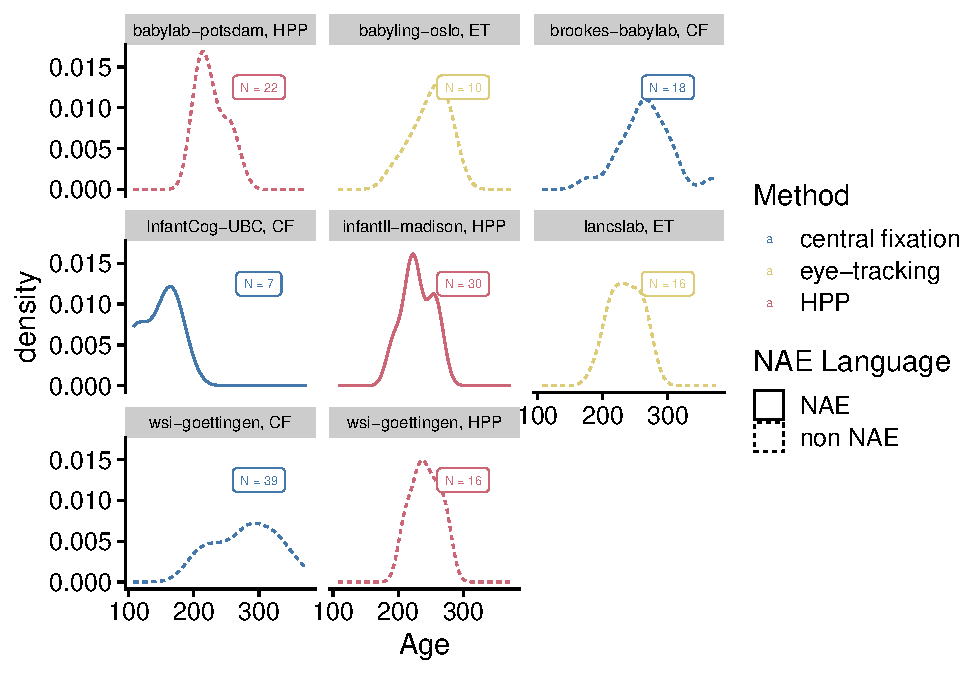
\includegraphics{MB1T_supplement_files/figure-latex/unnamed-chunk-3-1} 

}

\caption{Distribution of participant age for each lab and method. Method is highlighted by color and  language status is indicated by line type (solid = North American English; dashed = non-North American English).}\label{fig:unnamed-chunk-3}
\end{figure}

To highlight the distributions of the key moderators of interest, we include an additional plot representing the distribution of infant age among the 7 participating labs, split by method and language background (Figure 1).

\hypertarget{s2.1.2.-a-note-on-post-hoc-power}{%
\subsubsection{S2.1.2. A note on (post-hoc) power}\label{s2.1.2.-a-note-on-post-hoc-power}}

Our final sample size (\emph{N} = 158) --- although quite large for typical infant looking time studies --- had limited power to detect moderation effects. As a heuristic for approximate post-hoc power, we can consider the power to detect differences between correlations for our final sample. For the moderator of language background, we had \emph{n} = 37 participants with a North American English language background and \emph{n} =121 participants with non-North American English backgrounds. Given this sample size, differences between the two samples would have to be substantial in order to have reasonable power to detect a difference: assuming \emph{r} = 0 for one sample, we would only reach 80\% power to detect a difference if \emph{r} \textasciitilde{} 0.5 for the other sample. We had slightly more power to detect differences for method, where we had \emph{n} = 68 HPP observations and \emph{n} = 90 non-HPP observations. For example, again assuming \emph{r} = 0 for one sample, we would reach 80\% power to detect differences once \emph{r} \textasciitilde{} 0.43 for the second sample. Given the limited power to detect all but large effect sizes in our moderation analyses, we planned to treat any significant results from the moderator analyses with caution.

\hypertarget{s2.2.-time-between-test-sessions}{%
\subsection{S2.2. Time between test sessions}\label{s2.2.-time-between-test-sessions}}

\hypertarget{s2.2.1.-reliability-moderated-by-time-between-test-sessions}{%
\subsubsection{S2.2.1. Reliability moderated by time between test sessions}\label{s2.2.1.-reliability-moderated-by-time-between-test-sessions}}

The number of days between the first and second testing session varied widely across participants (mean: 10 days; range: 1 - 49 days). We therefore tested for the possibility that the time between sessions might have an impact on test-retest reliability. We fit a linear mixed-effects model predicting IDS preference in Session 2 from IDS preference in Session 1 (mean-centered), number of days between testing sessions (mean-centered), and their interaction, including a by-lab random intercept and random slope for IDS preference in Session 1.
A more complex random effects structure including additional random slopes for number of days between test sessions and its interaction with IDS preference in Session 1 did not converge.
We found no evidence that the number of days between test sessions moderated the relationship between IDS preference in Session 1 and 2. Neither the main effect of time between sessions, \(\beta\)=-0.01, \emph{SE}=0.03, \emph{t}(148.70)=-0.41, \emph{p}=.684, nor the interaction term, \(\beta\)=-0.01, \emph{SE}=0.02, \emph{t}(149.10)=-0.73, \emph{p}=.465, showed significant effects.

\hypertarget{s2.2.2.-change-in-preferential-looking-moderated-by-time-between-test-sessions}{%
\subsubsection{S2.2.2. Change in preferential looking moderated by time between test sessions}\label{s2.2.2.-change-in-preferential-looking-moderated-by-time-between-test-sessions}}

In addition to assessing the influence of moderators on test-retest reliability, we also tested whether the difference in magnitude of the IDS preference between Session 1 and Session 2 depended on moderators of interest.
To investigate the influence of time between test sessions, we fit a linear mixed-effects model predicting average IDS preference from Session (centered; Session 1 vs.~Session 2), days between test sessions (mean-centered), and their interaction.
We included by-lab and by-participant random intercepts (more complex random effects structures did not converge due to singular fits).
There were two key results.
We found no evidence that the change in preferential looking to IDS between Session 1 and Session 2 was moderated by days between test sessions, \(\beta\)=-0.02, \emph{SE}=0.04, \emph{t}(156)=-0.48, \emph{p}=.634.

\hypertarget{s2.3.-participant-age}{%
\subsection{S2.3. Participant age}\label{s2.3.-participant-age}}

\hypertarget{s2.3.1.-reliability-moderated-by-participant-age}{%
\subsubsection{S2.3.1. Reliability moderated by participant age}\label{s2.3.1.-reliability-moderated-by-participant-age}}

To investigate the possibility that age moderated test-retest reliability, we fit a linear mixed-effects model predicting IDS preference in Session 2 from IDS preference in Session 1 (mean-centered), participant age (mean-centered) and their interaction.
The model included a by-lab random intercept and a by-lab random slope for IDS preference in Session 1.
We found no evidence that age influenced test-retest reliability as indicated by the interaction between IDS preference in Session 1 and age, \(\beta\)=0.00, \emph{SE}=0.00, \emph{t}(76.60)=-0.85, \emph{p}=.398.

\hypertarget{s2.3.2.-change-in-preferential-looking-moderated-by-participant-age}{%
\subsubsection{S2.3.2. Change in preferential looking moderated by participant age}\label{s2.3.2.-change-in-preferential-looking-moderated-by-participant-age}}

To investigate the potential of moderators to influence the overall magnitude of the IDS effect between Session 1 and 2, we fit a linear mixed-effects model predicting average IDS preference from Session (centered; Session 1 vs.~Session 2), participant age (mean-centered), and their interaction.
We included by-lab and by-participant random intercepts (more complex random effects structures did not converge due to singular fits).
We found no evidence that the change in preferential looking to IDS between Session 1 and Session 2 was moderated by participant age, \(\beta\)=0.00, \emph{SE}=0.00, \emph{t}(157.50)=-0.56, \emph{p}=.577.

\hypertarget{s2.4.-method}{%
\subsection{S2.4. Method}\label{s2.4.-method}}

\hypertarget{s2.4.1.-ids-preference-moderated-by-method}{%
\subsubsection{S2.4.1. IDS preference moderated by method}\label{s2.4.1.-ids-preference-moderated-by-method}}

In ManyBabies1, infants who participated in the headturn preference procedure showed a significantly larger magnitude of IDS preference, compared to central fixation and eye-tracking methods. Therefore, in the current study, we also explored whether the magnitude of IDS preference differed as a function of method. We fit a linear mixed-effects model predicting IDS preference from Session and Method (dummy-coded, with central fixation as the reference level), including by-lab and by-participant random intercepts. We found no significant difference in IDS preference across methods, \({\chi}^2\)=1.11, \emph{p}=.575.

\hypertarget{s2.4.2.-reliability-moderated-by-method}{%
\subsubsection{S2.4.2. Reliability moderated by method}\label{s2.4.2.-reliability-moderated-by-method}}

We tested whether method (eye-tracking vs.~central fixation vs.~headturn preference procedure) moderated test-retest reliability by fitting a linear mixed-effects model predicting IDS preference in Session 2 from IDS preference in Session 1 (mean-centered), Method (dummy-coded, with central fixation as the reference level) and their interaction.
The model included a by-lab random intercept and a by-lab random slope for IDS preference in Session 1 (models with more complex random effects structure including by-lab random effects for Method did not converge).
We found no evidence that Method influenced test-retest reliability as indicated by the interaction between IDS preference in Session 1 and age, \({\chi}^2\)=3.85, \emph{p}=.146.

\hypertarget{s2.4.3.-reliability-and-its-interaction-with-both-method-and-age}{%
\subsubsection{S2.4.3. Reliability and its interaction with both method and age}\label{s2.4.3.-reliability-and-its-interaction-with-both-method-and-age}}

In a more complex linear mixed-effects model (preregistered as part of our planned secondary analyses) including the interaction between IDS preference in Session 1 (mean-centered), Method (dummy-coded, with central fixation as the reference level), participant age (mean-centered), and all lower order interactions, we find evidence for an interaction between method and age in predicting reliability, \({\chi}^2\)=6.44, \emph{p}=.040.
This effect appears to be mainly driven by older infants showing some evidence of test-retest reliability for the headturn preference procedure, \emph{r} = 0.45, \emph{p} = 0.02 (see Figure 3B).
However, we believe these tentative findings should be treated with caution, due to the small size of our infant sample once binned by multiple moderating factors.

\hypertarget{s2.4.4.-change-in-preferential-looking-moderated-by-age-and-method}{%
\subsubsection{S2.4.4. Change in preferential looking moderated by age and method}\label{s2.4.4.-change-in-preferential-looking-moderated-by-age-and-method}}

We fit a linear mixed-effects model predicting average IDS preference from the three-way interaction of Session (centered; Session 1 vs.~Session 2), participant age (mean-centered), Method (dummy-coded, with central fixation as the reference level) and all lower order predictors.
We included a by-participant random intercept (more complex random effects structures did not converge due to singular fits).
We found no evidence that the change in preferential looking to IDS between Session 1 and Session 2 was moderated by participant age and Method, \(\beta\)=-0.01, \emph{SE}=0.02, \emph{t}(155.40)=-0.58, \emph{p}=.562.

\hypertarget{s2.5.-language-background}{%
\subsection{S2.5. Language background}\label{s2.5.-language-background}}

\hypertarget{s2.5.1.-reliability-moderated-by-language-background}{%
\subsubsection{S2.5.1. Reliability moderated by language background}\label{s2.5.1.-reliability-moderated-by-language-background}}

\begin{figure}
\centering
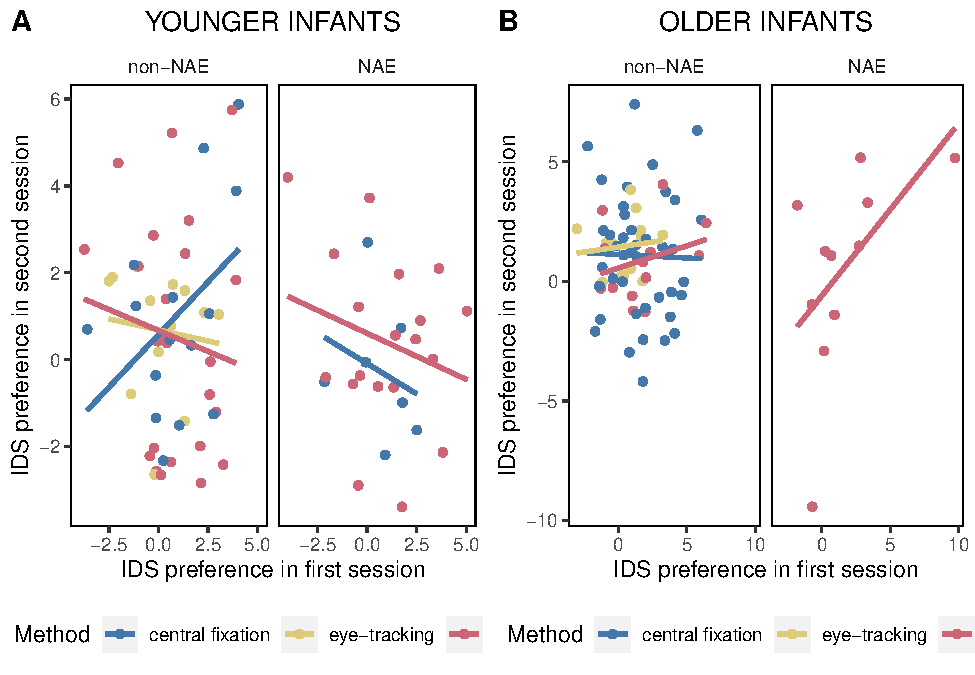
\includegraphics{MB1T_supplement_files/figure-latex/unnamed-chunk-15-1.pdf}
\caption{\label{fig:unnamed-chunk-15}Infants' preference in Session 1 and Session 2 with individual data points and regression lines color-coded by method (CF, ET, or HPP). Results are plotted separately for North American English-learning infants (right panel) and infants learning other languages and dialects (left panel).}
\end{figure}

NAE-learning infants showed greater IDS preferences than their non-NAE counterparts in MB1.
We therefore also assessed whether test-retest reliability interacted with children's language background.
A linear mixed-effects model predicting IDS preference in Session 2 based on IDS preference in Session 1 (mean-centered), NAE (centered), and their interaction, including Lab as a random intercept, revealed no interaction, \(\beta\)=0.29, \emph{SE}=0.18, \emph{t}(151.30)=1.59, \emph{p}=.115 (Figure 2).

\hypertarget{s2.5.2.-reliability-and-its-interaction-between-language-background-and-age}{%
\subsubsection{S2.5.2. Reliability and its interaction between language background and age}\label{s2.5.2.-reliability-and-its-interaction-between-language-background-and-age}}

\begin{figure}
\centering
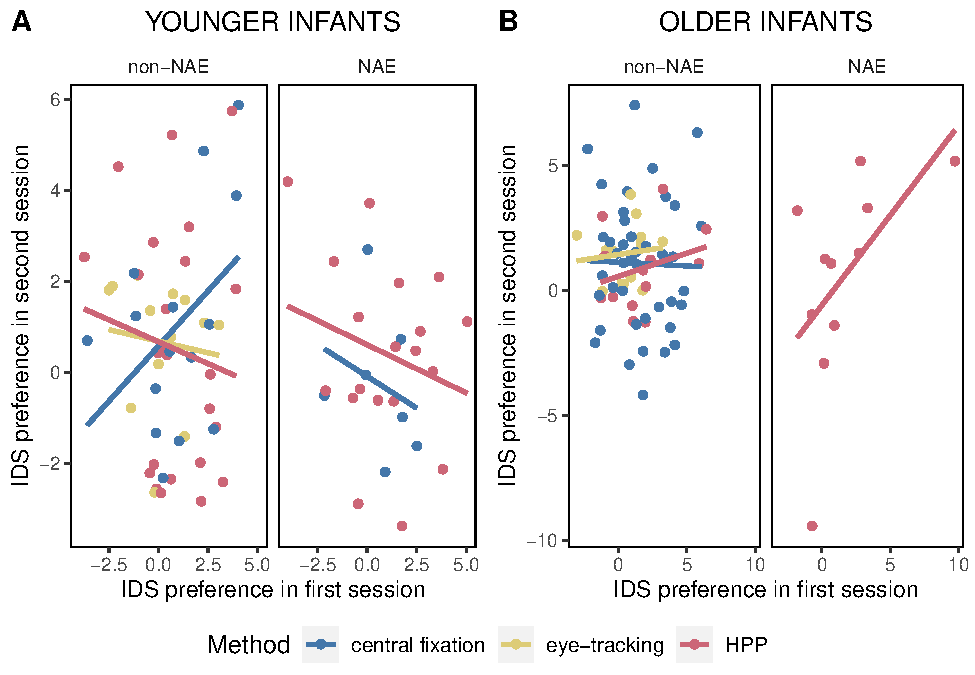
\includegraphics{MB1T_supplement_files/figure-latex/unnamed-chunk-17-1.pdf}
\caption{\label{fig:unnamed-chunk-17}Infants' preference in Session 1 and Session 2 with individual data points and regression lines color-coded by method for (A) younger and (B) older infants (median-split). Results are plotted separately for North American English-learning infants and infants learning other languages and dialects}
\end{figure}

We also fit a preregistered linear mixed-effects model predicting IDS preference in Session 2 from the three-way interaction between IDS preference in Session 1 (mean-centered), NAE (centered), participant age (mean-centered), and all lower order interactions.
We find evidence for an interaction between language background and age in predicting reliability, \(\beta\)=0.01, \emph{SE}=0.00, \emph{t}(63.70)=2.43, \emph{p}=.018.
Figure 3 illustrates that this interaction was driven by a small set of older infants (all from a single lab and participating in the HPP method) showing a somewhat more reliable relationship between Session 1 and Session 2 looking.
Note that the mixed-effects analyses use Age as a continuous predictor --- age is median-split in Figure 3 to ease visualization.
Given the small number of infants driving the three-way interaction and the confounded nature of this sample (with method and lab), we do not draw strong conclusions from the existence of this three-way interaction, but report it here to spur future investigations into how age and experience interacts with test-retest reliability.

\hypertarget{s2.5.3.-change-in-preferential-looking-moderated-by-age-and-language-background}{%
\subsubsection{S2.5.3. Change in preferential looking moderated by age and language background}\label{s2.5.3.-change-in-preferential-looking-moderated-by-age-and-language-background}}

We fit a linear mixed-effects model predicting average IDS preference from the three-way interaction of Session (centered; Session 1 vs.~Session 2), participant age (mean-centered), NAE (centered), and all lower order predictors.
We included by-lab and by-participant random intercepts and by-lab random slope for Session (more complex random effects structures did not converge due to singular fits).
We found no evidence that the change in preferential looking to IDS between Session 1 and Session 2 was moderated by participant age and language background, \(\beta\)=0.01, \emph{SE}=0.02, \emph{t}(114.60)=0.95, \emph{p}=.347.

\hypertarget{s3.-meta-analysis-of-test-retest-reliability}{%
\section{S3. Meta-analysis of test-retest reliability}\label{s3.-meta-analysis-of-test-retest-reliability}}

\begin{figure}
\centering
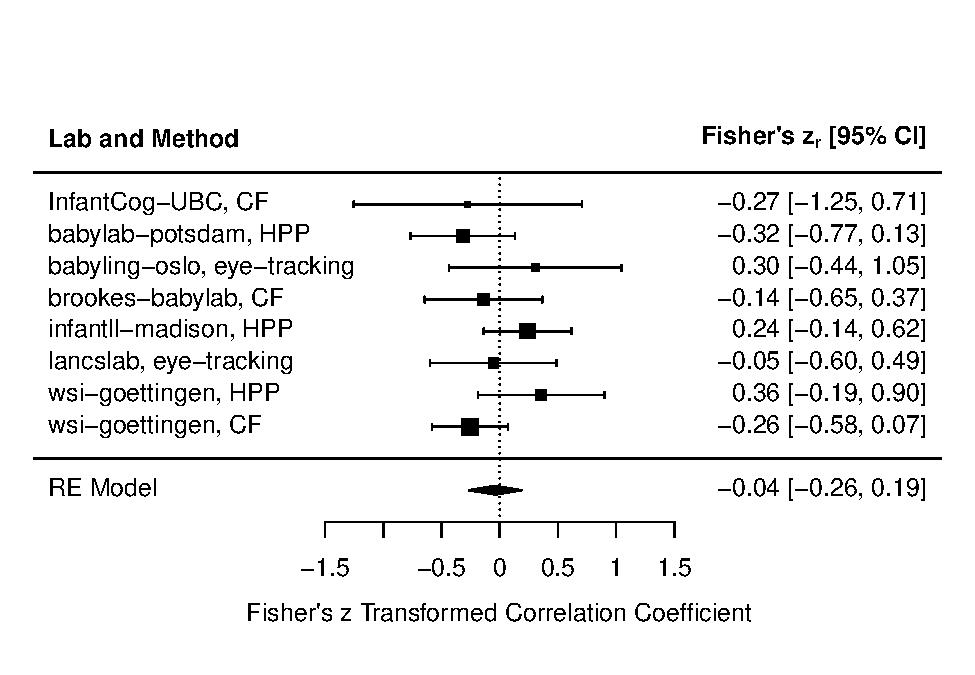
\includegraphics{MB1T_supplement_files/figure-latex/unnamed-chunk-20-1.pdf}
\caption{\label{fig:unnamed-chunk-20}Forest plot of test-retest reliability effect sizes. Each row represents Fisher's z transformed correlation coefficient and 95\% CI for a given lab and method (HPP = head-turn preference procedure; ET = eye-tracking; CF = central fixation). The black diamond represents the overall estimated effect size from the mixed-effects meta-analytic model.}
\end{figure}

In addition to the methods for assessing test-retest reliability reported in the main manuscript, we also investigated test-retest reliability across labs using a meta-analytic approach.
We used the metafor package (Viechtbauer, 2010) to fit a mixed-effects meta-analytic model on z-transformed correlations for each combination of lab and method using sample size weighting.
The model included random intercepts for lab and method.
The overall effect size estimate was not significantly different from zero, \emph{b} = -0.04, 95\% CI = {[}-0.26, 0.19{]}, \emph{p} = 0.73.
A forest plot of the effect sizes for each lab and method is shown in Figure 4.

\hypertarget{s4.-analyses-including-a-more-restricted-sample}{%
\section{S4. Analyses including a more restricted sample}\label{s4.-analyses-including-a-more-restricted-sample}}

Given that we found that restricting the sample to participants contributing at least 6 ADS and IDS trials in both sessions, we conducted the central analyses with this more restricted infant sample.

\hypertarget{s4.1.-descriptives-and-ids-preference-for-the-restricted-sample}{%
\subsection{S4.1. Descriptives and IDS preference for the restricted sample}\label{s4.1.-descriptives-and-ids-preference-for-the-restricted-sample}}

\begin{table}[tbp]

\begin{center}
\begin{threeparttable}

\caption{\label{tab:labs6}Statistics of the included labs for the restricted sample (min 6 trials contributed per session). N refers to the number of infants included in the analysis.}

\begin{tabular}{lllll}
\toprule
Lab & \multicolumn{1}{c}{Method} & \multicolumn{1}{c}{Language} & \multicolumn{1}{c}{Mean age (days)} & \multicolumn{1}{c}{N}\\
\midrule
InfantCog-UBC & central fixation & English & 136 & 5\\
babylab-potsdam & HPP & German & 224 & 18\\
babyling-oslo & eye-tracking & Norwegian & 250 & 1\\
brookes-babylab & central fixation & English & 254 & 15\\
infantll-madison & HPP & English & 233 & 12\\
lancslab & eye-tracking & English & 235 & 10\\
wsi-goettingen & HPP & German & 240 & 13\\
wsi-goettingen & central fixation & German & 281 & 26\\
\bottomrule
\end{tabular}

\end{threeparttable}
\end{center}

\end{table}

The participants in the restricted sample --- contributing at least 6 IDS and ADS trials for both sessions --- were distributed across the contributing labs, methods, and language backgrounds (Table 2). There was no difference in average age between the main sample and the restricted sample (\(t(204.57) = -0.33\), \(p = .744\)). There was a robust preference for infant-directed speech in both session 1 (\(t(99) = 6.67\), \(p < .001\)) and session 2 (\(t(99) = 4.42\), \(p < .001\)). We observed no difference in IDS preference between the two sessions, \(\beta\)=-0.34, \emph{SE}=0.28, \emph{p}=.225.

Interestingly, while there was a significant simple correlation between IDS preference in session 1 and session 2 (\(r = .22\), 95\% CI \([.02, .40]\), \(t(98) = 2.23\), \(p = .028\)), we found that IDS preference in session 1 did not significantly predict IDS preference in session 2 in a linear mixed-effects model including a by-lab random intercept, \(\beta\)=0.12, \emph{SE}=0.11, \emph{p}=.255.

\hypertarget{s4.2.-moderator-analyses-including-a-more-restricted-sample}{%
\subsection{S4.2. Moderator analyses including a more restricted sample}\label{s4.2.-moderator-analyses-including-a-more-restricted-sample}}

\hypertarget{s4.2.1.-time-between-test-sessions}{%
\subsubsection{S4.2.1. Time between test sessions}\label{s4.2.1.-time-between-test-sessions}}

As in the analyses with the full dataset, we found no evidence that the number of days between test sessions moderated the relationship between IDS preference in Session 1 and 2. Neither the main effect of time between sessions, \(\beta\)=-0.03, \emph{SE}=0.03, \emph{t}(95.80)=-0.96, \emph{p}=.342, nor the interaction term, \(\beta\)=-0.01, \emph{SE}=0.03, \emph{t}(93.60)=-0.22, \emph{p}=.828, showed significant effects.

\hypertarget{s4.2.2.-participant-age}{%
\subsection{S4.2.2. Participant age}\label{s4.2.2.-participant-age}}

To investigate the possibility that age moderated test-retest reliability in the restricted sample, we fit a linear mixed-effects model predicting IDS preference in Session 2 from IDS preference in Session 1 (mean-centered), participant age (mean-centered) and their interaction.
The model included a by-lab random intercept and a by-lab random slope for IDS preference in Session 1.
We found no evidence that age influenced test-retest reliability as indicated by the interaction between IDS preference in Session 1 and age, \(\beta\)=0.00, \emph{SE}=0.00, \emph{t}(43.20)=-0.69, \emph{p}=.494.

\hypertarget{s4.2.3.-method}{%
\subsection{S4.2.3. Method}\label{s4.2.3.-method}}

We tested whether method (eye-tracking vs.~central fixation vs.~headturn preference procedure) moderated test-retest reliability by fitting a linear mixed-effects model predicting IDS preference in Session 2 from IDS preference in Session 1 (mean-centered), Method (dummy-coded, with central fixation as the reference level) and their interaction.
The model included a by-lab random intercept and a by-lab random slope for IDS preference in Session 1.
We found no evidence that Method influenced test-retest reliability as indicated by the interaction between IDS preference in Session 1 and age, \({\chi}^2\)=3.85, \emph{p}=.146. There was no significant relationship between IDS preference for session 1 and session 2 for each method considered separately (central fixation:\(\beta\)=-0.06, \emph{SE}=0.16, \emph{p}=.704; HPP: \(\beta\)=0.26, \emph{SE}=0.17, \emph{p}=.139; eye-tracking: \(\beta\)=-0.04, \emph{SE}=0.26, \emph{p}=.866)

\hypertarget{s4.2.4.-language-background}{%
\subsection{S4.2.4. Language background}\label{s4.2.4.-language-background}}

As in the main sample, a linear mixed-effects model predicting IDS preference in Session 2 based on IDS preference in Session 1 (mean-centered), NAE (centered), and their interaction, including Lab as a random intercept, revealed no interaction, \(\beta\)=0.31, \emph{SE}=0.24, \emph{t}(95.10)=1.29, \emph{p}=.199.

\newpage

\hypertarget{s5.-alternative-dependent-variables}{%
\section{S5. Alternative dependent variables}\label{s5.-alternative-dependent-variables}}

To check the robustness of our results, we also investigated whether we obtained similar results with other possible dependent measures: average log-transformed looking times and a proportion-based preference measure. For each alternative dependent variable, we conducted the main analyses of test-retest reliability reported in the manuscript: the overall Pearson correlation, the test-retest linear mixed-effects model, and an inspection of applying stricter inclusion criteria for number of trials contributed.

\hypertarget{s5.1.-correlations-between-alternative-dependent-variables}{%
\subsection{S5.1. Correlations between alternative dependent variables}\label{s5.1.-correlations-between-alternative-dependent-variables}}

\begin{table}[tbp]

\begin{center}
\begin{threeparttable}

\caption{\label{tab:unnamed-chunk-29}Correlations between alternative dependent measures}

\begin{tabular}{lllll}
\toprule
 & \multicolumn{1}{c}{1} & \multicolumn{1}{c}{2} & \multicolumn{1}{c}{M} & \multicolumn{1}{c}{SD}\\
\midrule
1. Diff & - &  & 1.21 & 2.22\\
2. Prop & .96*** & - & 0.54 & 0.07\\
3. Diff\_log\_lt & .95*** & .96*** & 0.16 & 0.30\\
\bottomrule
\addlinespace
\end{tabular}

\begin{tablenotes}[para]
\normalsize{\textit{Note.} * p < 0.05; ** p < 0.01; *** p < 0.001}
\end{tablenotes}

\end{threeparttable}
\end{center}

\end{table}

First, we consider the correlations between the three dependent measures we considered for IDS preference: (a) a simple difference score between average IDS and ADS looking times (main manuscript), (b) a difference score between average log-transformed looking times, and (c) the proportion-based preference measure. As expected, the correlations between the alternative dependent measures was very high (all \emph{r}s \textgreater{} 0.95; Table 3).

\hypertarget{s5.2.-log-transformed-looking-times}{%
\subsection{S5.2. Log-transformed looking times}\label{s5.2.-log-transformed-looking-times}}

\begin{table}[tbp]

\begin{center}
\begin{threeparttable}

\caption{\label{tab:unnamed-chunk-31}Coefficient estimates from a linear mixed-effects model predicting Log LT IDS preference in Session 2.}

\begin{tabular}{lllll}
\toprule
 & \multicolumn{1}{c}{Estimate} & \multicolumn{1}{c}{SE} & \multicolumn{1}{c}{t} & \multicolumn{1}{c}{p}\\
\midrule
Intercept & 0.14 & 0.07 & 2.05 & 0.09\\
Log LT IDS Preference Session 1 & -0.06 & 0.09 & -0.68 & 0.50\\
\bottomrule
\end{tabular}

\end{threeparttable}
\end{center}

\end{table}

\begin{figure}

{\centering 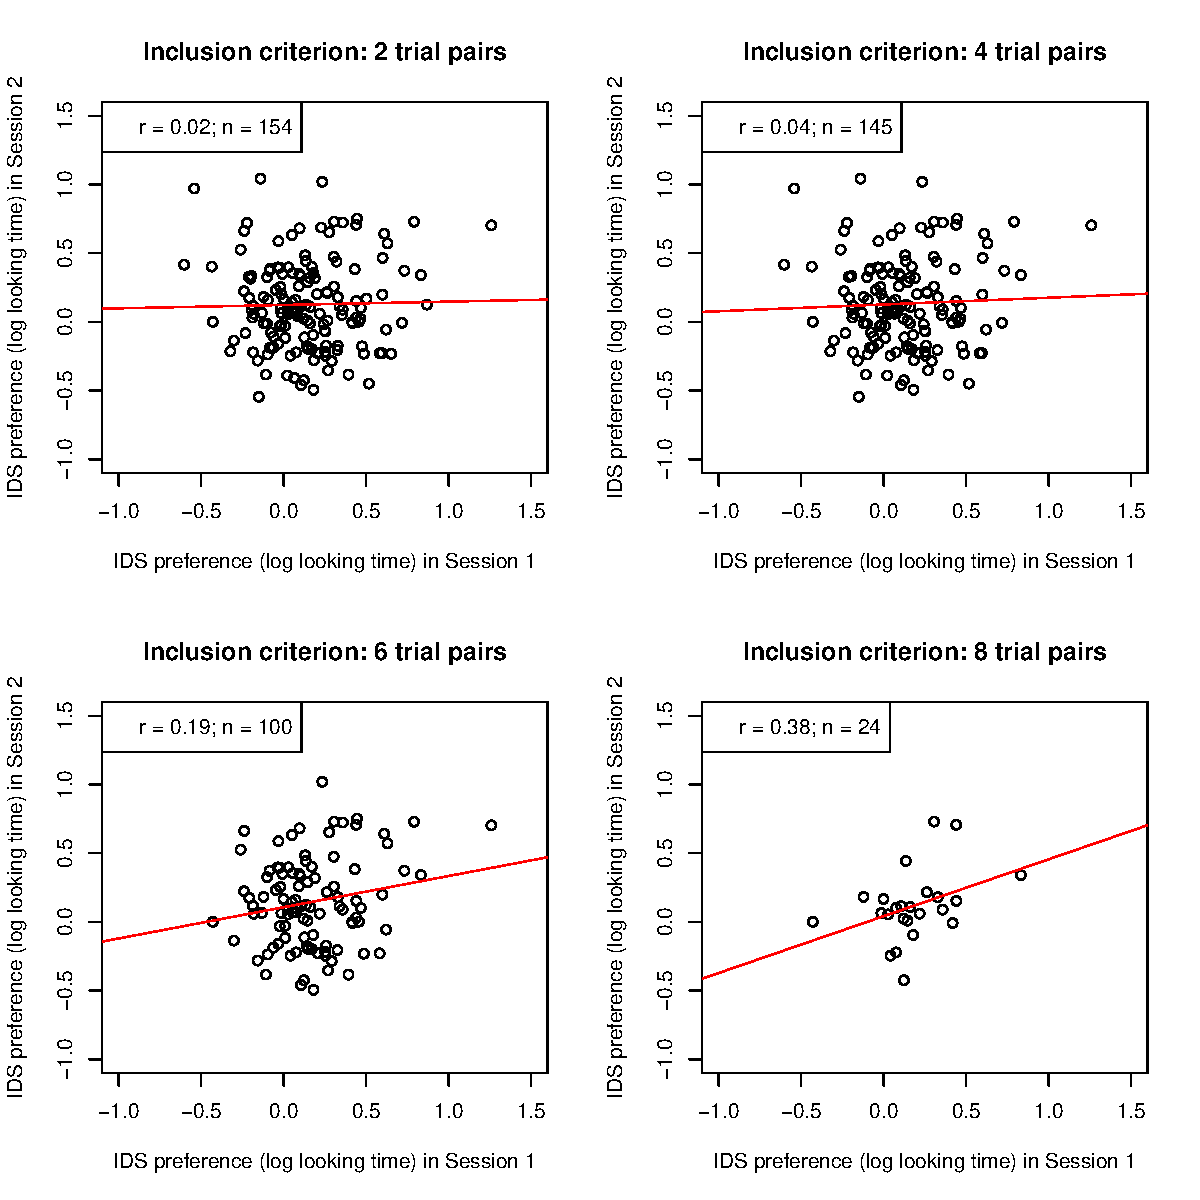
\includegraphics[width=5in]{MB1T_supplement_files/figure-latex/unnamed-chunk-32-1} 

}

\caption{IDS preferences (based on average log-looking times) of both sessions plotted against each other for each inclusion criterion. n indicates the number of included infants, r is the Pearson correlation coefficient as the indicator for reliability.}\label{fig:unnamed-chunk-32}
\end{figure}

In these analyses, we calculated IDS preference by first log-transforming looking times for each trial, computing the average log-transformed looking time for IDS and ADS for each participant, and calculating the difference between average IDS and ADS log-transformed looking times.
We fit a linear mixed-effects model predicting IDS preference in Session 2 from IDS preference in Session 1, including a by-lab random intercept.
As in the analyses using average raw looking times, the results revealed no significant relationship between IDS preference in Session 1 and 2 (Table 4).
The Pearson correlation coefficient was also not statistically significant, \(r = .03\), 95\% CI \([-.12, .19]\), \(t(156) = 0.43\), \(p = .670\).
Applying successively stricter inclusion criteria --- by requiring a higher number of valid trials per condition in each session --- showed a similar pattern to the main manuscript, such that correlations increased somewhat with stricter inclusion criteria, but substantially reduced the sample size at the same time (Figure 5).

\hypertarget{s5.3.-proportion-looking-to-ids}{%
\subsection{S5.3. Proportion looking to IDS}\label{s5.3.-proportion-looking-to-ids}}

Next, we calculated a proportion-based IDS preference measure by computing the average proportion (raw) looking time to IDS relative to total (raw) looking time to IDS and ADS for each subject (i.e., IDS looking time / (ADS looking time + IDS looking time)).
We fit a linear mixed-effects model predicting proportion-based IDS preference in Session 2 from proportion-based IDS preference in Session 1, including a by-lab random intercept.
As in the analyses using other measures of IDS preference, the results revealed no significant relationship between IDS preference in Session 1 and 2 (Table 5).
The Pearson correlation coefficient based on proportional IDS looking was also not statistically significant, \(r = .01\), 95\% CI \([-.15, .16]\), \(t(156) = 0.09\), \(p = .927\).
Stricter inclusion criteria increased the correlation somewhat, as in previous analyses (Figure 6).

\begin{figure}

{\centering 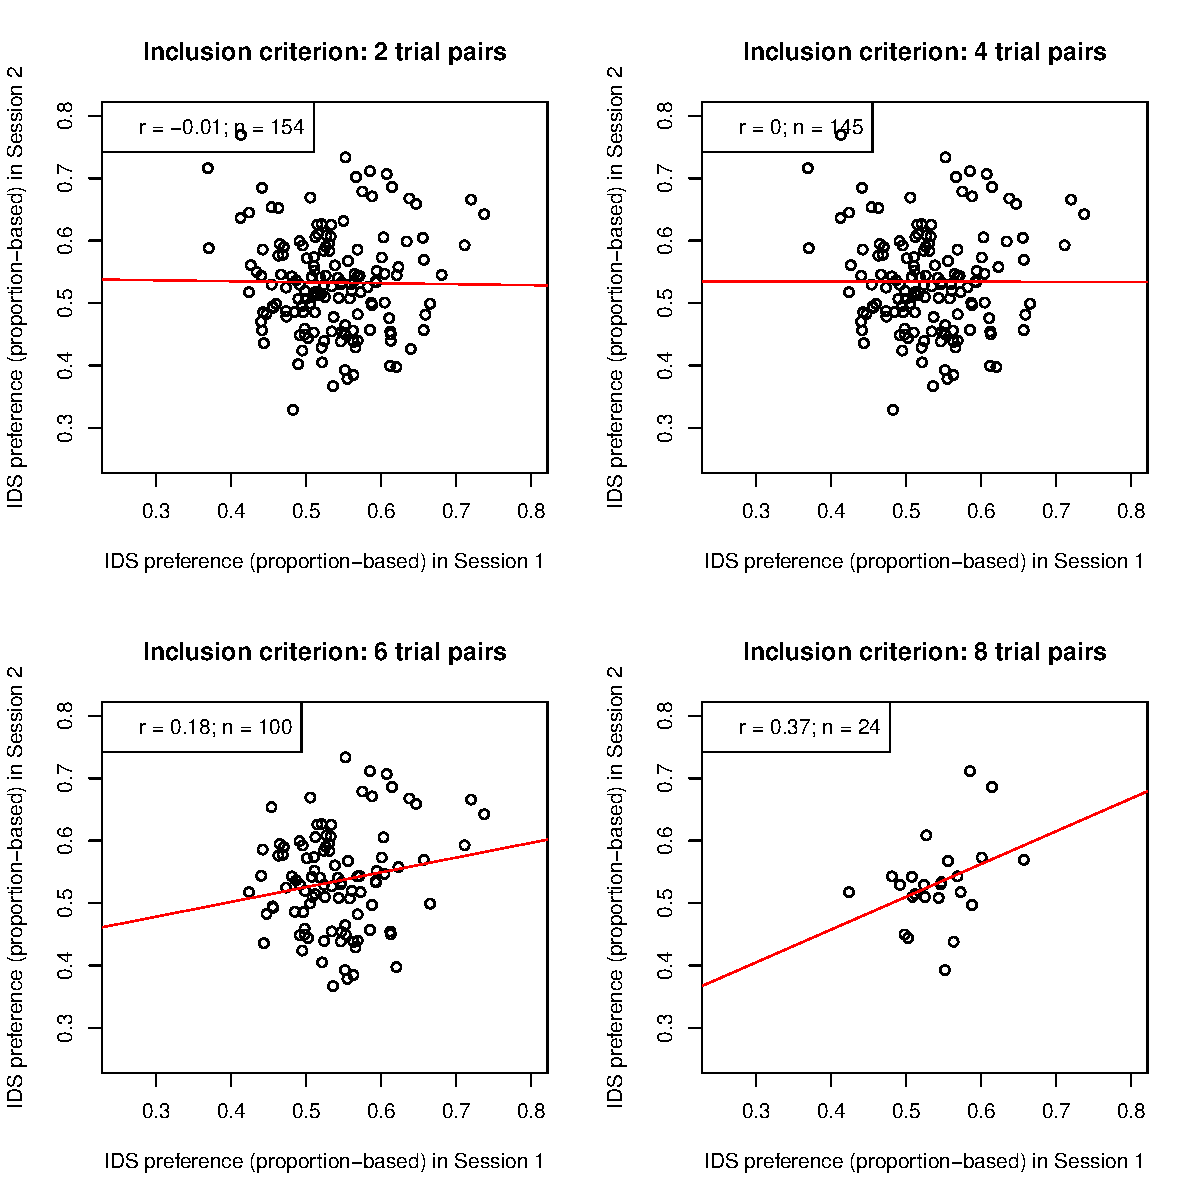
\includegraphics[width=5in]{MB1T_supplement_files/figure-latex/unnamed-chunk-34-1} 

}

\caption{IDS preferences (based on proportion IDS looking) of both sessions plotted against each other for each inclusion criterion. n indicates the number of included infants, r is the Pearson correlation coefficient as the indicator for reliability.}\label{fig:unnamed-chunk-34}
\end{figure}

\begin{table}[tbp]

\begin{center}
\begin{threeparttable}

\caption{\label{tab:unnamed-chunk-35}Coefficient estimates from a linear mixed-effects model predicting IDS preference (based on proportion IDS looking) in Session 2.}

\begin{tabular}{lllll}
\toprule
 & \multicolumn{1}{c}{Estimate} & \multicolumn{1}{c}{SE} & \multicolumn{1}{c}{t} & \multicolumn{1}{c}{p}\\
\midrule
Intercept & 0.59 & 0.05 & 10.70 & 0.00\\
IDS Preference (proportion measure) Session 1 & -0.10 & 0.10 & -1.01 & 0.31\\
\bottomrule
\end{tabular}

\end{threeparttable}
\end{center}

\end{table}

\newpage

\hypertarget{s6.-sensitivity-of-test-retest-reliability-to-trial-number-inclusion-criteria}{%
\section{S6. Sensitivity of test-retest reliability to trial number inclusion criteria}\label{s6.-sensitivity-of-test-retest-reliability-to-trial-number-inclusion-criteria}}

To conduct a more fine-grained analysis of how stricter trial inclusion criteria affect test-retest reliability, we computed correlations while gradually increasing the number of total valid trials required for inclusion.
For this analysis, we required a minimum of one IDS and one ADS trial and gradually increased the number of total valid trials required in both sessions (irrespective of IDS and ADS condition) from 2 to 16 (the maximum number of total trials).
Figure 7 depicts the Pearson correlation coefficients for increasingly stricter requirements for the overall trial numbers of a given participant in both sessions.
Correlations only increase and reach conventional levels of significance once the number of total required trials for both sessions is greater than 12.

\begin{figure}
\centering
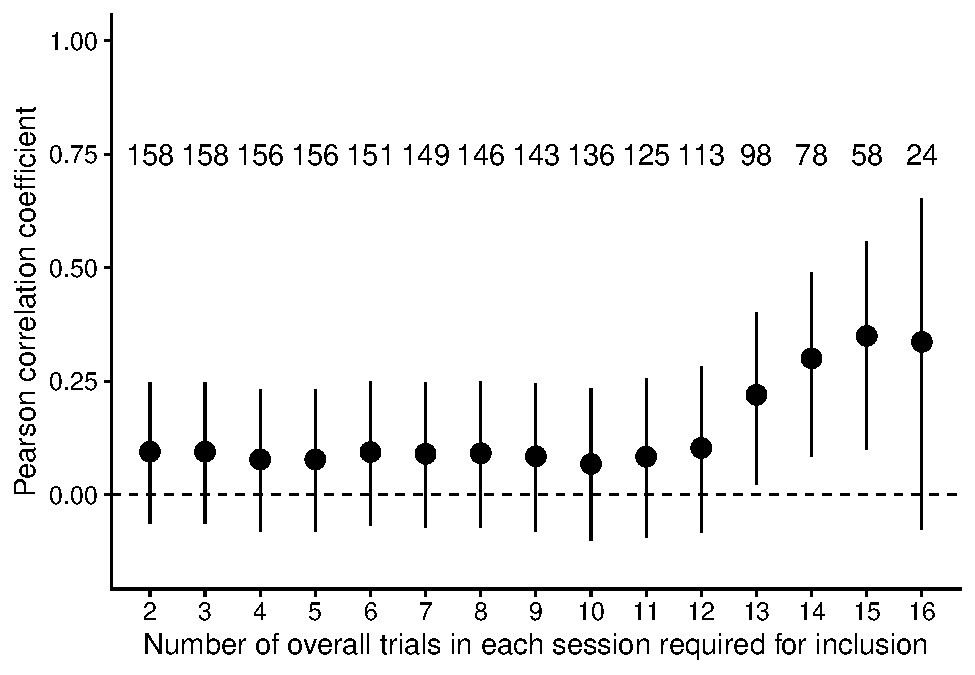
\includegraphics{MB1T_supplement_files/figure-latex/sfig7-1.pdf}
\caption{\label{fig:sfig7}Pearson correlation coefficient with increasingly strict trial-level inclusion criteria. The x-axis depicts the required number of overall valid trials in both session 1 and session 2. Dots represent corresponding correlation coefficients, with 95 percent CIs. The sample size is shown above each dot.}
\end{figure}

\newpage

\hypertarget{s7.-patterns-of-preference-across-sessions}{%
\section{S7. Patterns of preference across sessions}\label{s7.-patterns-of-preference-across-sessions}}

We also conducted analyses to explore whether there were any patterns of preference reversal across test sessions.
While there was no strong correlation in the magnitude of IDS preference between test session 1 and test session 2, here we asked whether infants consistently expressed the same preference across test sessions.
Overall, 58.20\% of the infants had a consistent preference from test to retest session.
Of the 158 total infants, 44.90\% of infants showed a consistent IDS preference and 13.30\% showed a consistent ADS preference.
23.40\% of infants switched from an IDS preference at test session 1 to an ADS preference at test session 2 and 18.40\% switched from an ADS preference to an IDS preference.

Next, we explored whether we could detect any systematic clustering of infants with distinct patterns of preference across the test and retest session.
We took a bottom-up approach and conducted a \emph{k}-means clustering of the test-retest difference data (here using log-transformed looking time data).
We found little evidence of distinct clusters emerging from these groupings: the clusterings ranging from \emph{k}=2 (2 clusters) to \emph{k}=4 (4 clusters) appear to mainly track whether participants are approximately above or below the mean looking time difference for test session 1 and test session 2 (Figure 8A).
The diagnostic elbow plot shows little evidence of a qualitative improvement as the number of clusters is increased, which suggests little evidence for a distinctive set of clusters of participants who showed similar patterns of looking across the test and retest sessions (Figure 8B).

\begin{figure}
\centering
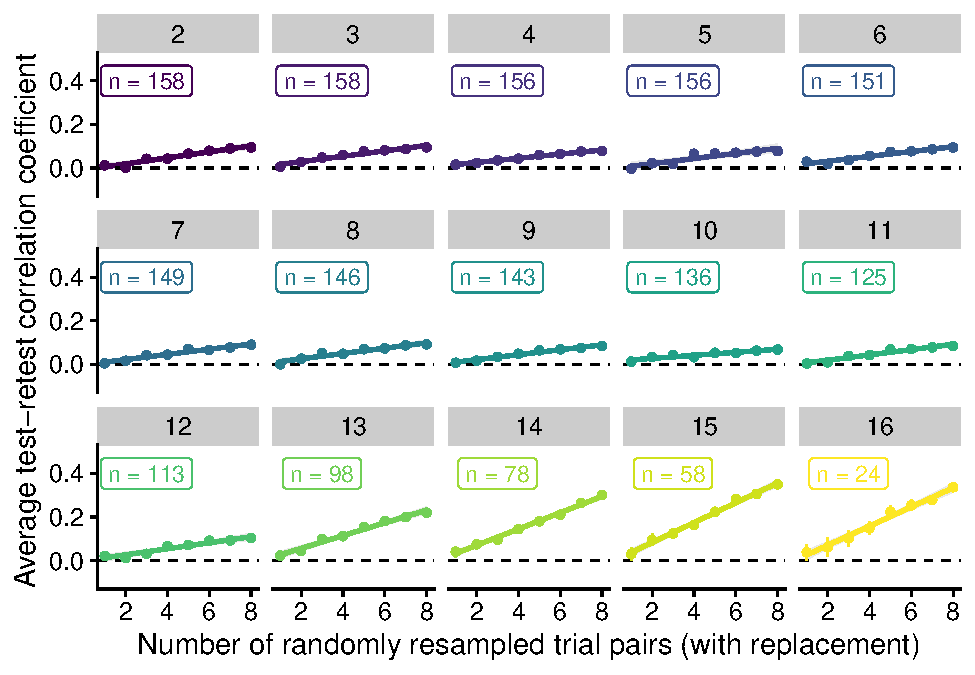
\includegraphics{MB1T_supplement_files/figure-latex/fig8-1.pdf}
\caption{\label{fig:fig8} (A) Results from the k-means clustering analysis of IDS preference (based on average log looking times) in session 1 and 2 for different numbers of k and (B) the corresponding elbow plot of the total within-cluster sum of squares. In (A), points represent indvidual participants' magnitude of looking time difference at test sessions 1 (x-axis) and 2 (y-axis). The solid line indicates no preference for IDS vs.~ADS, the dotted lines indicate mean IDS preference at test session 1 and 2, respectively. Colors indicate clusters from the k-means clustering for different values of k.}
\end{figure}

\newpage

\hypertarget{s8.-relation-between-number-of-contributed-trials-in-each-session}{%
\section{S8. Relation between number of contributed trials in each session}\label{s8.-relation-between-number-of-contributed-trials-in-each-session}}

\begin{figure}
\centering
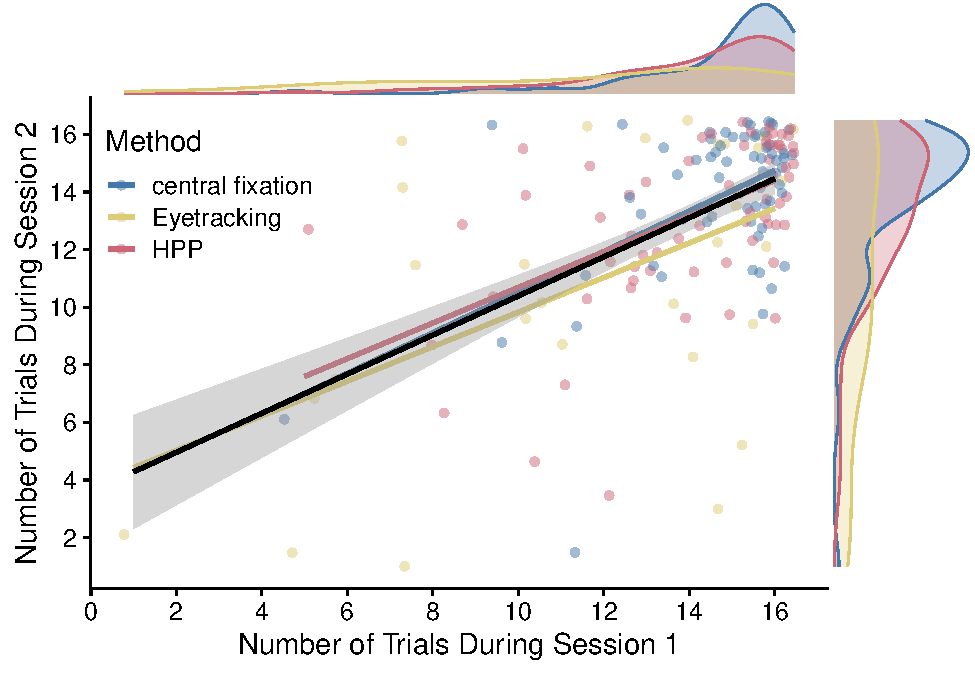
\includegraphics{MB1T_supplement_files/figure-latex/sfig9-1.pdf}
\caption{\label{fig:sfig9}Correlation between the number of trials contributed in Session 1 and Session 2. Each data point represents one infant. Colored lines represent linear fits for each method.}
\end{figure}

Are there stable individual differences in how likely an infant is to contribute a high number of trials?
To answer this question, we conducted an exploratory analysis investigating whether there is a relationship between the number of trials an infant contributed in Session 1 and Session 2.
Do infants who contribute a higher number of trials during their first testing session also tend to contribute more trials during their second testing session?
A positive correlation between trial numbers during the first and second session would indicate that there is some stability in a given infants' likelihood of remaining attentive throughout the experiment.
On the other hand, the absence of a correlation would indicate that the number of trials a given infant contributes is not predictive of how many trials they might contribute during their next session.

We found a strong positive correlation between number of trials contributed during the first and the second session \(r = .58\), 95\% CI \([.47, .67]\), \(t(160) = 9.00\), \(p < .001\) (Figure 9).
This result suggests that if infants contribute a higher number of trials in one session, compared to other infants, they are likely to contribute a higher number of trials in their next session.
This finding is consistent with the hypothesis that how attentive infants are throughout an experiment (and hence how many trials they contribute) is a stable individual difference, at least for some infant looking time tasks.
Researchers should therefore be mindful of the fact that decisions about including or excluding infants based on trials contributed may selectively sample a specific sub-set of the infant population they are studying (Byers-Heinlein, Bergmann, \& Savalei, 2021; DeBolt, Rhemtulla, \& Oakes, 2020).

\newpage

\hypertarget{s9.-correlations-in-average-looking-times-between-sessions}{%
\section{S9. Correlations in average looking times between sessions}\label{s9.-correlations-in-average-looking-times-between-sessions}}

To what extent are participants looking times between the two sessions related?
To test this question, we first investigated whether participants' overall looking times --- irrespective of condition --- were correlated between the first and second session.
There was a robust correlation between average looking time in Session 1 and Session 2: infants with longer looking times during their first session also tended to look longer during their second session, \(r = .45\), 95\% CI \([.31, .57]\), \(t(156) = 6.28\), \(p < .001\).
This relationship held even after controlling for number of trials in the first and second session, suggesting that the relation between average looking in Session 1 and 2 could not be entirely explained by the correlation in the number of trials contributed between the two sessions (S7), \(b = 0.42\), 95\% CI \([0.27, 0.58]\), \(t(154) = 5.52\), \(p < .001\) (Figure 10A).
The result is also similar when controlling for participants' average age across the two test sessions, \(b = 0.44\), 95\% CI \([0.30, 0.59]\), \(t(155) = 6.16\), \(p < .001\).

Next, we explored the extent to which average looking times for IDS and ADS stimuli were related.
First, we found similar correlations in average looking time to IDS stimuli in Session 1 and 2, \(r = .38\), 95\% CI \([.24, .51]\), \(t(156) = 5.19\), \(p < .001\), and ADS stimuli in Session 1 and 2, \(r = .40\), 95\% CI \([.26, .53]\), \(t(156) = 5.49\), \(p < .001\) (Figure 10B).
To test whether these correlations were specific to looking times for IDS or ADS stimuli alone, we fit linear regression models predicting average looking to IDS (or ADS) stimuli in Session 2 from average looking to IDS and ADS stimuli in Session 1.
We found that average looking to IDS stimuli in Session 2 could be predicted from average looking to IDS stimuli in Session 1, even after controlling for average looking to ADS stimuli in Session 1, \(b = 0.21\), 95\% CI \([0.01, 0.41]\), \(t(155) = 2.11\), \(p = .037\).
Conversely, average looking to ADS stimuli in Session 2 could be predicted from average looking to ADS stimuli in Session 1, even after controlling for average looking to IDS stimuli in Session 1, \(b = 0.36\), 95\% CI \([0.14, 0.58]\), \(t(155) = 3.20\), \(p = .002\).
These results suggest that the condition-specific correlations in average looking time cannot be fully explained by the fact that infants' overall looking times between sessions are correlated.

Finally, we inspected item-level correlations between the two test sessions.
Specifically, we investigated the relation between items composed of the same recording clips in Session 1 and Session 2 (but with a reversed order of clips between the two sessions).
We fit a linear mixed-effects model predicting item-level looking time in Session 2 from item-level looking time in Session 1, including random intercepts for participant, item, and lab, as well as a random slope for item-level looking time in Session 1 for participant and lab.
Item-level looking in Session 2 was related to item-level looking in Session 1, \(\hat{\beta} = 0.17\), 95\% CI \([0.07, 0.27]\), \(t(5.52) = 3.38\), \(p = .017\) (Figure 10C).
Similar results hold if looking times are log-transformed.

In ManyBabies1, the ordering of stimuli was counterbalanced, but some stimuli still appeared earlier in the experiment than others. For example, the IDS1 and ADS1 speech stimuli appeared on trials 1,2,5, or 6, while the IDS8 and ADS8 speech stimuli always occurred on the final two trials (trial number 15 or 16). This means that the interpretation of the correlations between individual speech stimuli must also take into account these stimuli tend to be occurring in earlier or later portions of the experiment (when infants are more or less attentive and show longer looking times in general). To further investigate the impact of trial number on by-item correlations in looking time, we fit an interaction model testing whether the magnitude of the item-level correlation depended on the trial number for a given session. We fit a linear mixed-effects predicting item-level looking time in Session 2 from the interaction between item-level looking time in Session 1 and trial number in Session 1 (trial numbers across sessions are almost always identical). The model included random intercepts for participant, item, and lab, as well as random slopes for item-level looking time and trial number in Session 1 for participant and lab. We indeed found that the magnitude of the item-level correlations in looking time between sessions depended on trial number (\(\hat{\beta} = -0.01\), 95\% CI \([-0.02, 0.00]\), \(t(1,200.31) = -2.53\), \(p = .012\)), with the strength of the relation between sessions declining as trial number increased. While trial number was a strong predictor of Session 2 looking time (\(\hat{\beta} = -0.28\), 95\% CI \([-0.36, -0.20]\), \(t(8.67) = -6.85\), \(p < .001\)), item-level looking in Session 1 only marginally predicted Session 2 looking when controlling for trial number (\(\hat{\beta} = 0.10\), 95\% CI \([0.01, 0.20]\), \(t(6.47) = 2.12\), \(p = .075\)). Variation in item-level correlations is therefore at least partially due to the ordering of the stimuli in the experiment, rather than a sole function of differences between the stimuli \emph{per se}.

\begin{figure}

{\centering 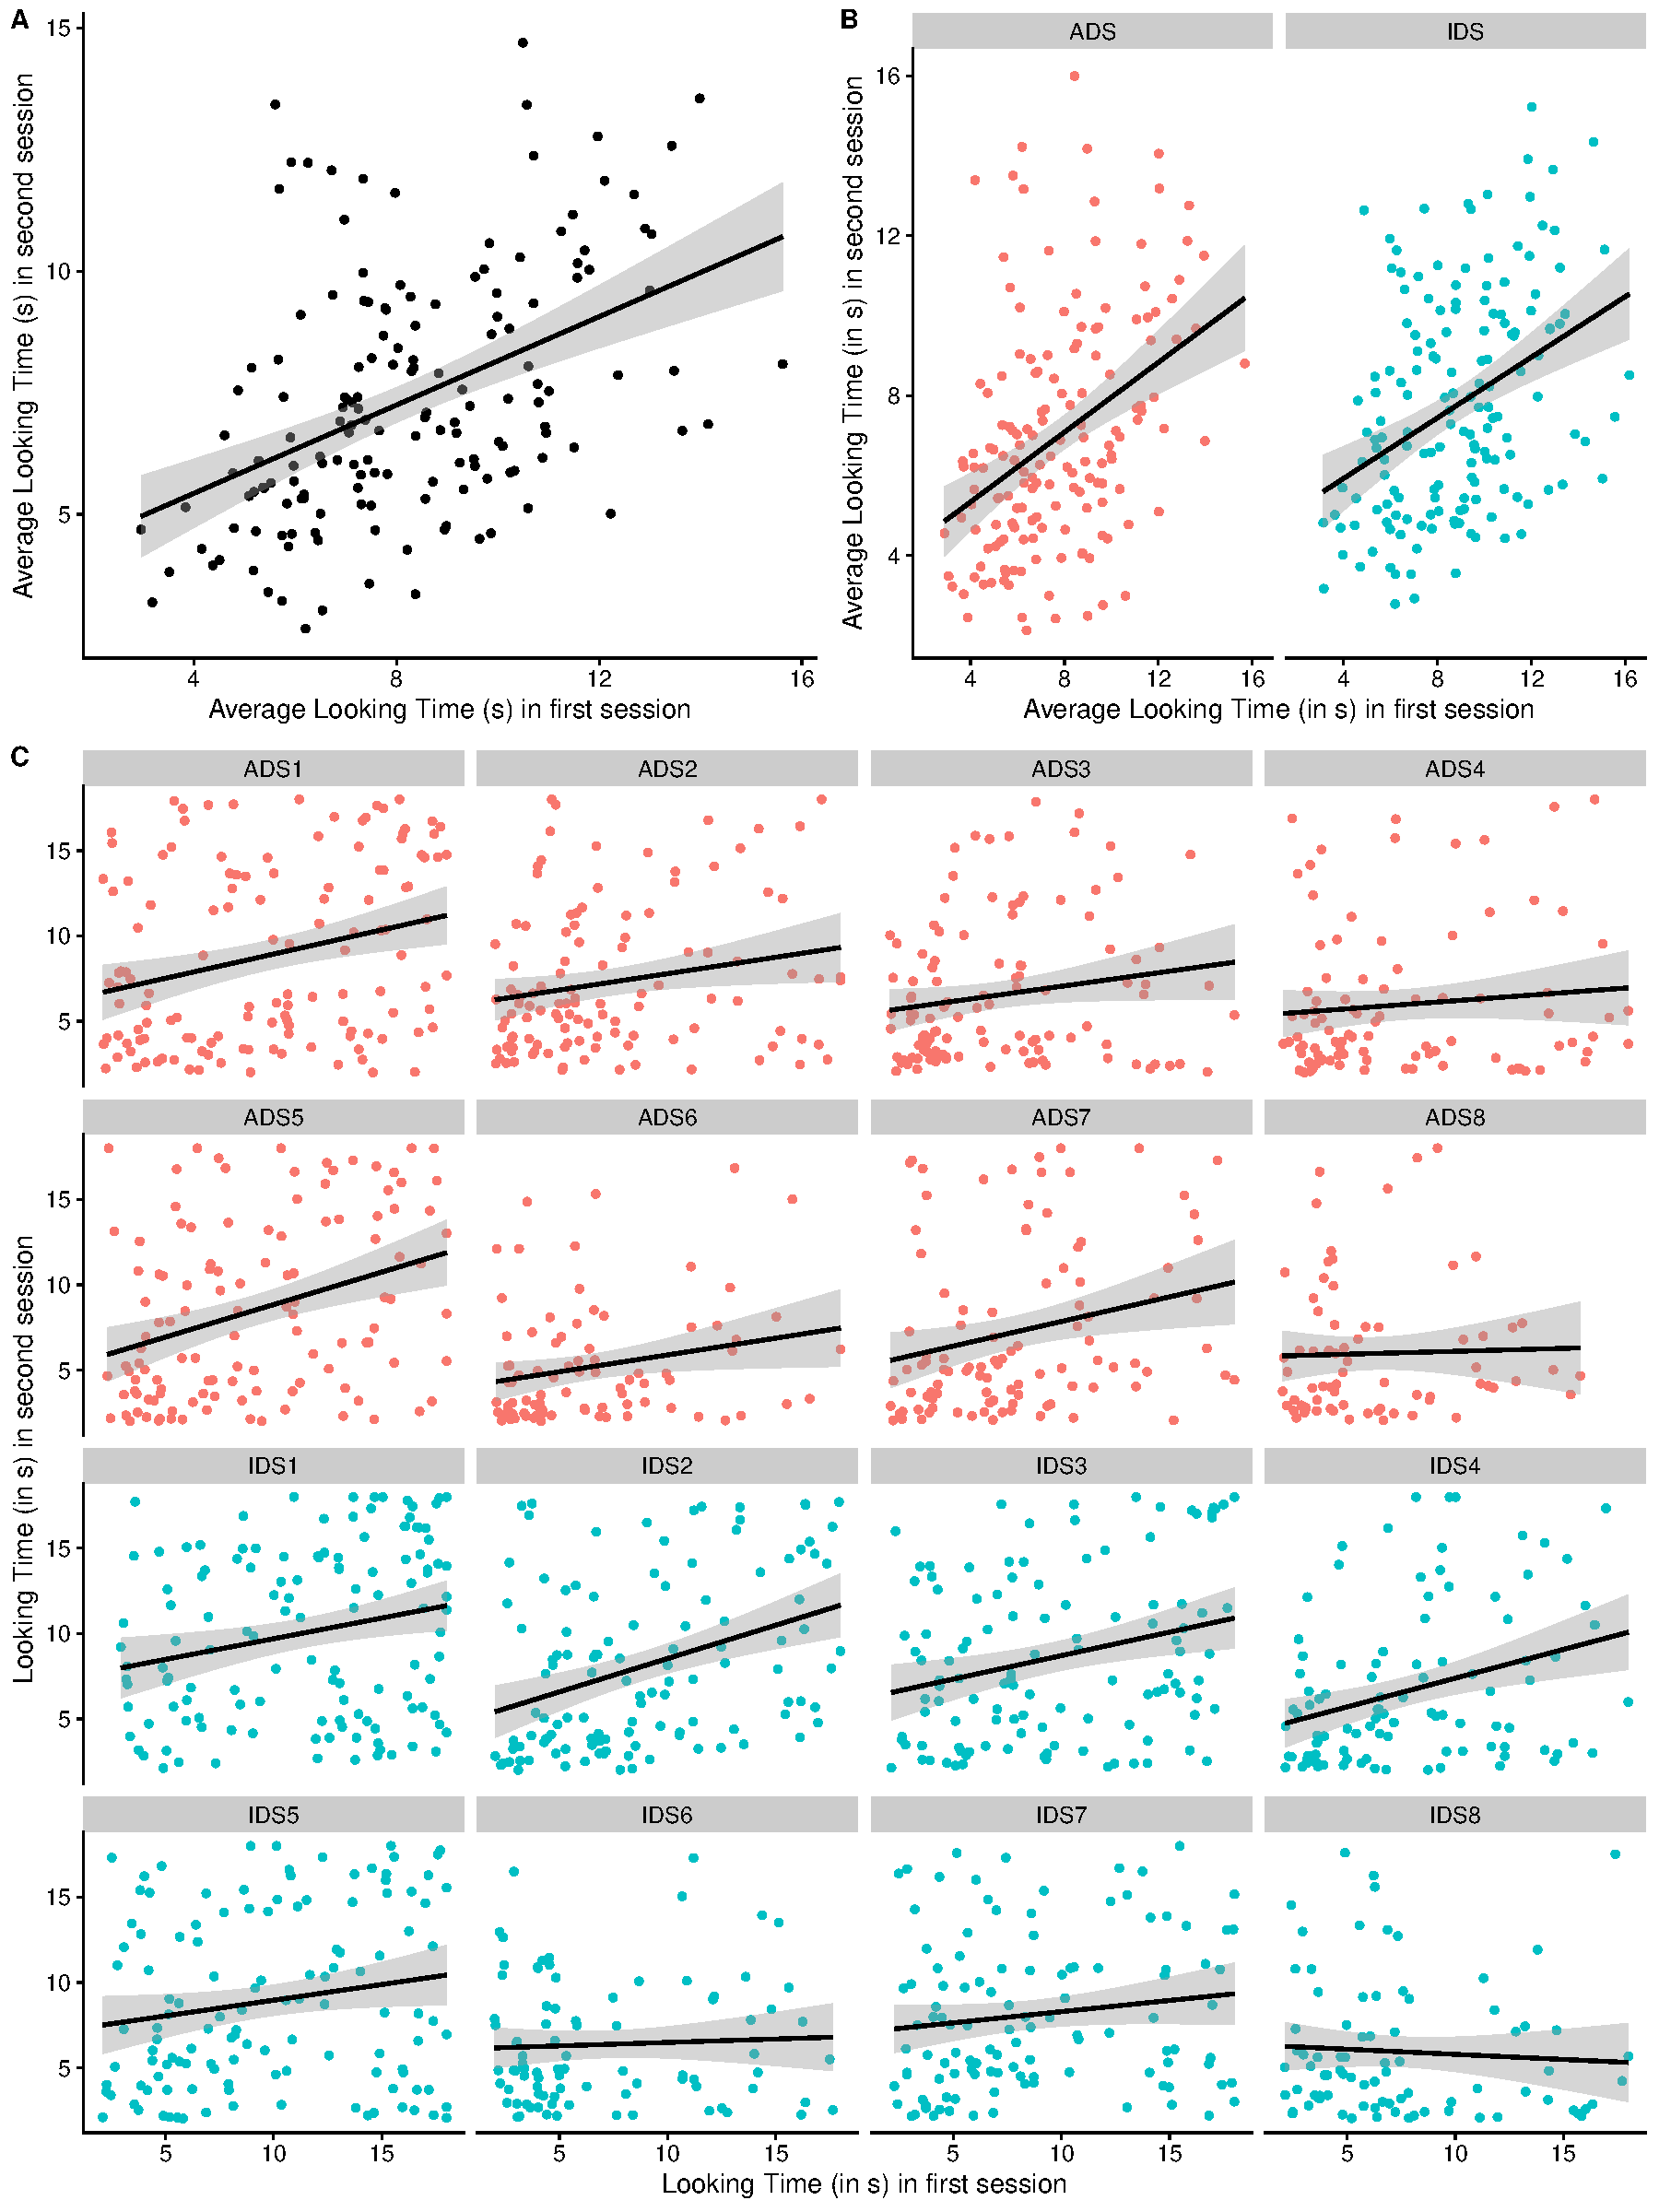
\includegraphics{MB1T_supplement_files/figure-latex/sfig10-1} 

}

\caption{Correlations in average looking time (in s) between Session 1 and 2 (A) overall, (B) by condition, and (C) by item.}\label{fig:sfig10}
\end{figure}

\newpage

\hypertarget{s10.-by-item-pair-preference-scores-across-sessions}{%
\section{S10. By-item-pair preference scores across sessions}\label{s10.-by-item-pair-preference-scores-across-sessions}}

Finally, we inspected on a more fine-grained item level whether IDS preference in Session 1 was related to IDS preference in Session 2.
To do so, we exploited the fact the specific IDS and ADS stimuli were paired together in test orders in both sessions, such that one IDS stimulus (e.g., IDS1) always occurred adjacently to a specific ADS stimulus (e.g., ADS1).
We therefore computed stimulus-specific IDS preference scores by calculating the difference in raw looking time for each of the eight IDS-ADS stimulus pairs for each participant (whenever both trials in a given pair were available).
We then fit a linear mixed-effects model predicting stimulus-specific IDS preference in Session 2 from stimulus-specific IDS preference in Session 1, including by-participant and by-lab random intercepts (models with more complex random effects structure, including by-item random effects, failed to converge).
There was a marginal, but non-significant relation in stimulus-specific IDS preference between the two test sessions (Table 6).

\begin{table}[tbp]

\begin{center}
\begin{threeparttable}

\caption{\label{tab:unnamed-chunk-44}Linear mixed-effects model results predicting IDS preference in Session 2 from IDS preference in Session 1 at the stimulus level.}

\begin{tabular}{llllll}
\toprule
Term & \multicolumn{1}{c}{$\hat{\beta}$} & \multicolumn{1}{c}{95\% CI} & \multicolumn{1}{c}{$t$} & \multicolumn{1}{c}{$\mathit{df}$} & \multicolumn{1}{c}{$p$}\\
\midrule
Intercept & 1.02 & {}[0.14, 1.90] & 2.27 & 6.55 & .060\\
Diff 1 & 0.07 & {}[-0.01, 0.14] & 1.79 & 718.46 & .074\\
\bottomrule
\end{tabular}

\end{threeparttable}
\end{center}

\end{table}

\newpage

\hypertarget{references}{%
\section{References}\label{references}}

\begingroup
\setlength{\parindent}{-0.5in}
\setlength{\leftskip}{0.5in}

\hypertarget{refs}{}
\begin{CSLReferences}{1}{0}
\leavevmode\vadjust pre{\hypertarget{ref-byers2021six}{}}%
Byers-Heinlein, K., Bergmann, C., \& Savalei, V. (2021). Six solutions for more reliable infant research. \emph{Infant and Child Development}, e2296.

\leavevmode\vadjust pre{\hypertarget{ref-debolt2020robust}{}}%
DeBolt, M. C., Rhemtulla, M., \& Oakes, L. M. (2020). Robust data and power in infant research: A case study of the effect of number of infants and number of trials in visual preference procedures. \emph{Infancy}, \emph{25}(4), 393--419.

\leavevmode\vadjust pre{\hypertarget{ref-manybabies2020quantifying}{}}%
ManyBabies Consortium. (2020). Quantifying sources of variability in infancy research using the infant-directed-speech preference. \emph{Advances in Methods and Practices in Psychological Science}, \emph{3}(1), 24--52.

\leavevmode\vadjust pre{\hypertarget{ref-R-metafor}{}}%
Viechtbauer, W. (2010). Conducting meta-analyses in {R} with the {metafor} package. \emph{Journal of Statistical Software}, \emph{36}(3), 1--48. Retrieved from \url{https://doi.org/10.18637/jss.v036.i03}

\end{CSLReferences}

\endgroup


\end{document}
